\subsection{Transformation of Bayer to YCbCr 4:2:0}
Three steps are needed to Transform the Bayer data to YCbCr 4:2:0; values from the bayer we first perform debayeiring using the \gls{mhc} coefficients in Figure \ref{fig:debayer:malvar_filters}, perform a linear mapping to get the YCbCr and finally perform chroma subsampling to get the 4:2:0 format.
For each \gls{cg} this results in four Y walues, one Cb value and one Cr value.



\begin{figure}[H]
    \centering
    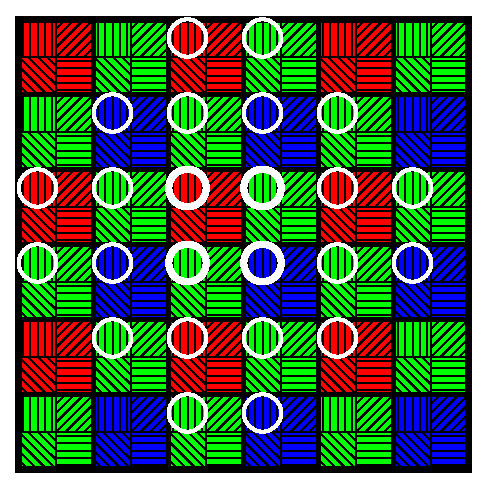
\includegraphics[width=.5\textwidth]{figures/polarized_image/normal_conv.pdf}
    \caption{Visualization of which pixels are used (white cirle) to calculate 6 YCbCr 4:2:0 values for the center \gls{cg} (thick white cirle).}
    \label{fig:saperation}
\end{figure}

This operation was performed algebraicly using \gls{sympy} and it was discovered that it could be formulated as sequence of \gls{fma} operations.

In order to achieve the high throughput, \gls{sympy} was used to analyse the algebraic expressions for the transformation from bayer data to YCbCr and a custom code generator was written to generate the corresponding CUDA code.


By calculating the four Y values, Cb and Cr values directly for each \gls{cg} we can save





As both the debayering and color space conversion consists exclusively of linear operations it is possible to combine them into a single operation.


How this is done to calculate one Y value is visualized in Figure \ref{fig:saperation}.



\begin{table}[H]
    \begin{minipage}[b]{.5\linewidth}
        \subcaptionbox{Separate debayering and color space conversion. Also shows where synchronization would be needed.}{
            \small
            \begin{tabular}{|l|c| c|}
                \hline
                \textbf{Operation}                         & \textbf{\# of \acrshort{fma}} \\
                \hline
                Green at red            (\ref{fig:mhc_gr}) & 9                             \\
                Green at blue           (\ref{fig:mhc_gb}) & 9                             \\
                Red at green 1 (\ref{fig:mhc_rgr})         & 11                            \\
                Red at green 2 (\ref{fig:mhc_rgb})         & 11                            \\
                Red at blue             (\ref{fig:mhc_rb}) & 9                             \\
                Blue at green 1 (\ref{fig:mhc_bgr})        & 11                            \\
                Blue at green 2 (\ref{fig:mhc_bgb})        & 11                            \\
                Blue at red             (\ref{fig:mhc_br}) & 9                             \\
                \textbf{\textit{Synchronize}}              &                               \\
                Convert to YCbCr                           & 36                            \\
                \textbf{\textit{Synchronize}}              &                               \\
                Binning Cb                                 & 4                             \\
                Binning Cr                                 & 4                             \\
                \hline
                \textbf{Total}                             & 124                           \\
                \hline
            \end{tabular}}
    \end{minipage}
    \begin{minipage}[b]{.5\linewidth}
        \subcaptionbox{Joined debayering and color space conversion.}{
            \small
            \begin{tabular}{|l|c|}
                \hline
                \textbf{Operation} & \textbf{\# of \acrshort{fma}} \\
                \hline
                Y at red           & 13                            \\
                Y at green 1       & 13                            \\
                Y at green 2       & 13                            \\
                Y at blue          & 13                            \\
                Cb                 & 24                            \\
                Cr                 & 24                            \\
                \hline
                \textbf{Total}     & 100                           \\
                \hline
            \end{tabular}}
    \end{minipage}
    \caption{Comparison of the number of \gls{fma} operations required to get the desired output. On the left }
\end{table}



\begin{listing}[H]
    \begin{minted}{cuda}
        __device__ __forceinline__ __half2 handle_u(__half2 **data, int col) {
            __half2 tmp = __float2half2_rn(5.000000000e-1f);
            tmp = __hfma2(__float2half2_rn(9.466415405e-5f), data[1][col + 1], tmp);
            tmp = __hfma2(__float2half2_rn(9.466415405e-5f), data[3][col - 1], tmp);
        \end{minted}
    \vspace{-26pt}
    \begin{minted}[linenos=false, autogobble=false]{cuda}
    ...
    \end{minted}
    \vspace{-26pt}
    \begin{minted}[firstnumber=24]{cuda}
        tmp = __hfma2(__float2half2_rn(-1.122532265e-5f), data[0][col], tmp);
        tmp = __hfma2_sat(__float2half2_rn(-1.122532265e-5f), data[2][col - 2], tmp);
        return __hfma2(__float2half2_rn(1023.0f), tmp, __float2half2_rn(0.0f));
    }
    \end{minted}
    \caption{Generated function}
    \label{listing:generated_function}
\end{listing}